\documentclass{llncs}

\usepackage{graphicx}
\usepackage{placeins}
\usepackage{algorithm}
\usepackage[noend]{algpseudocode}
\usepackage{amssymb}
\usepackage{listings}

\begin{document}

\title{Optimization of String Rewriting Operations for 3D Fractal Generation with Genetic Algorithms}

\author{Todor Balabanov, Janeta Sevova, Kolyu Kolev}

% Todor Balabanov todorb@iinf.bas.bg
% Kolyu Kolev kolev_kolyu@yahoo.com
% Janeta Sevova janetasevova@gmail.com

\institute{Institute of Information and Communication Technologies \\
Bulgarian Academy of Sciences \\
acad. Georgi Bonchev Str., block 2, office 514, 1113 Sofia, Bulgaria \\
\email{todorb@iinf.bas.bg} \\
\texttt{http://www.iict.bas.bg/}}

%----------------------------------------------------------------------------------------
%   Title
%----------------------------------------------------------------------------------------
\maketitle

%----------------------------------------------------------------------------------------
%   Abstract
%----------------------------------------------------------------------------------------
\begin{abstract}
String rewriting is a modification of the idea for the context-free grammar. Modification consists in the fact that there is not separation on terminal and nonterminal symbols. Each symbol in string rewriting, is considered as nonterminal and it can produce longer sequence. By this way infinite structures are created as fractals. In a video presentation by Jack Hodkinson the use of 2D images instead of text symbol pixels is suggested. Each pixel (geometric square) is divided in nine sub-squares. The color of the pixel determine the pattern in which the nine squares are arranged. By this way each pixel gives a rule for subdivision of the containing area. Hodkinson gives a method, to setup the fractal, to reproduce a particular 2D image (for example, the glyph of the Greek letter $\pi$). This problem is well known in the fractals theory as Fractal Inverse Problem (FIP). It is an optimization problem, so a good option is the use of genetic algorithm (GA), to assemble set of rules, for string rewriting with 2D pixels. Series of experiments with the size of substitution matrix (not only 3x3, but also 2x2 and 4x4) are done by Hodkinson. Also are made series of experiments with different number of colors, starting with black/white and reaching the final successful experiment with thirty shades of blue. In this study the idea for string rewriting is extended in the 3D space and instead of pixels voxels are used with 3x3x3 substitution matrix. The study is only on virtual models but with the usage of industrial tomography, 3D objects can be scanned and with 3D color printer generated fractals can be printed.
\keywords{fractal inverse problem, genetic algorithms, string rewriting}
\end{abstract}

%----------------------------------------------------------------------------------------
%   Paper
%----------------------------------------------------------------------------------------
\section{Introduction} \label{Introduction}

This study addresses IFP which is well known in the fractals theory \cite{guerin01,nettleton01}. There is a branch in the theory for the formal languages which is related to a context-free grammar (CFG). In such grammar there are set of production rules. Application of these rules, lead to generation of all possible strings in a specified formal language \cite{ochoa01}. In CFG, a production rule is an operation of simple replacement. Rules are applied regardless of the context. The left hand side of a CFG rule is always nonterminal symbol. It means that nonterminal symbols are not part of the resulting string. The right hand side of a CFG rule, consists of terminal symbol, nonterminal symbols or combination of both. The main idea in CFGs is that nonterminal symbols are substituted with the given rules until there is no nonterminal symbols in the generated string.

String rewriting system (SRS) is a substitution system in which the rules does not contain nonterminal symbols. Each terminal symbol can appear on the left hand side (LHS) of the rule and on the right hand side (RHS) of the rule. With such definition SRS are useful for generation of infinite structures and they are mainly used for the generation of some fractals (for example: Box Fractal, Cantor Dust, Cantor Square Fractal and Sierpinski Carpet). Most of the fractals are generated with binary rules (black and white colors), but in the Hodkinson's research it is clearly shown that limit of the colors can be higher.

\begin{figure}[h!]
  \centering
  
\includegraphics[width=0.5\linewidth]{pic01}
  \caption{Fractal generated by Jack Hodkinson.}
\label{fig:pic01}
\end{figure}

The problem in 1D is well presented by \cite{shonkwiler01}, but in Hodkinson's research, the genetic algorithms (GAs) are used for 2D shape of Greek letter $\pi$, to be reconstructed with substitution rules of 30 shades of blue pixels (Fig. \ref{fig:pic01}). The usage of differential evolution is also applicable \cite{zelinka01}, but not in Hodkinson's research, because the optimization is in a discrete space.  The key problem in this research is which rules to be selected to achieved the final goal. GAs is a promising approach for such kind of combinatorial optimization. A single rule has LHS pixel with particular color and nine pixels on the RHS as 3x3 substitution matrix. Image starts with a single pixel and it grows on size by 3 on each iteration. 

This study extends the idea from 2D space into 3D space, which is the main contribution of the authors. Voxels are used instead of pixels. Square matrix of 3x3 is replaced with cube 3x3x3. The paper is organized as follows: Section \ref{Introduction} introduces the problem; Section \ref{Model and Optimization} presents a model and optimization approach; Section \ref{Experiments and Results} gives experiment details and the results are shown; Section \ref{Conclusions} concludes and some further ideas for research are pointed.

\section{Model and Optimization} \label{Model and Optimization}

A finite 3D space is represented as three-dimensional array of voxels in the model. Each voxel is encoded with a single long integer value, which consists of the RGB (red, green, blue) information for the color of the voxel. In this model 32 different transition 3x3x3 matrices are selected, each corresponding to the one of the 32 colors. The steps for fractal generation are given in Algorithm \ref{algorithm01}.

\begin{algorithm}
\caption{Fractal generation algorithm.}\label{algorithm01}
\begin{algorithmic}[1]
\Procedure{Generate}{$Level,Voxel$}
\If{$Level \leqslant 0$}
  \State return\label{alg:step04}
\EndIf
\State $v\gets Split(Voxel)$\label{alg:step01}
\For{each $v$}
  \State Paint($v$)\label{alg:step02}
  \State Generate($Leve$-1, $v$)\label{alg:step03}
\EndFor
\EndProcedure
\end{algorithmic}
\end{algorithm}
\FloatBarrier

The splitting of the voxel is done on 27 smaller voxels with 1/3 side size of the original Step \ref{alg:step01}. Each sub-voxel is painted according to the color of transition matrix pattern Step \ref{alg:step02}. A recursive call of generator procedure is done for each sub-voxel Step \ref{alg:step03}. Recursive generation of the fractal stops when the recursion level reached zero Step \ref{alg:step04}.

The individuals in the genetic algorithm are presented as 32 transition matrices each with size 3x3x3 (Listing \ref{listing03} in \cite{balabanov01}). Long integer numbers are used for RGB color representation for all 27 cells of the transition matrix. 

\begin{lstlisting}[language=Java, caption=Chromosomes encoding., label=listing03]
List<Chromosome> list = new LinkedList<Chromosome>();

for (int i = 0; i < 37; i++) {
	Long cells[] = new Long[COLORS.length * 3*3*3];
	
	for (int j = 0; j < cells.length; j++) {
		cells[j] = 
		COLORS[PRNG.nextInt(COLORS.length)];
	}
	
	list.add(new TransitionsChromosome(cells, 
	RECURSION_DEPTH, COLORS, target, start));
}
\end{lstlisting}

The order of the matrices shows which transition will be applied according to used colors order. The steps of the optimization are illustrated in Algorithm \ref{algorithm02}. 

\begin{algorithm}
\caption{Genetic algorithm.}\label{algorithm02}
\begin{algorithmic}[1]
\Procedure{Optimization}{}
\State $p \gets Initialize()$\Comment{Initialize population.}
\While{$TimeLimit > 0$}
  \State Selection($p$)\Comment{Select parents.}
  \State Crossover($p$)\Comment{Crossover parents.}
  \State Mutation($p$)\Comment{Mutate children.}
  \State Evaluation($p$)\Comment{Evaluate offspring.}
\EndWhile
\EndProcedure
\end{algorithmic}
\end{algorithm}
\FloatBarrier

Parents in the population are appointed by tournament selection with arity of two (Listing \ref{listing01} in \cite{balabanov01}). 

\begin{lstlisting}[language=Java, caption=Genetic algorithm parameters., label=listing01]
GeneticAlgorithm optimizer = new GeneticAlgorithm(
new UniformCrossover<TransitionsChromosome>(0.5), 0.9, 
new TransitionsMutation(COLORS), 0.01, 
new TournamentSelection(2));
\end{lstlisting}

Uniform crossover is taken as the most symmetric crossover (Listing \ref{listing01} in \cite{balabanov01}). From each parent randomly are taken 50\% of the elements. Random change of a color is used for the mutation operator (Listing \ref{listing02} in \cite{balabanov01}). 

\begin{lstlisting}[language=Java, caption=Color mutation of a single voxel., label=listing02]
List<Long> values = new 
ArrayList<Long>(((TransitionsChromosome) original).
getRepresentation());

values.set(PRNG.nextInt(values.size()), 
colors[PRNG.nextInt(colors.length)]);
\end{lstlisting}

The evaluation is done by application of each 32 transition matrices with the certain level of recursion depth. As suggested in \cite{guerin01}, an Euclidean distance between generated fractal and target shape is used as fitness function (Listing \ref{listing04} in \cite{balabanov01}). 

\begin{lstlisting}[language=Java, caption=Euclidean distance between voxels., label=listing04]
double result = 0;
for (int x = 0; x < a.length && 
		x < b.length; x++)
for (int y = 0; y < a[x].length && 
		y < b[x].length; y++)
for (int z = 0; z < a[x][y].length && 
		z < b[x][y].length; z++)
result += (a[x][y][z] - b[x][y][z]) * 
	(a[x][y][z] - b[x][y][z]);

result = Math.sqrt(result);
\end{lstlisting}

The initial fractal is a single cube painted with the color with the first index in the order of the colors. Genetic algorithms are global heuristics optimization and this means that it does not matter what kind of color the initial voxel will have. 

\section{Experiments and Results} \label{Experiments and Results}

All experiments are done in Java programming language with Apache Genetic Algorithms Framework \cite{apache01} as an optimization approach and Printing in 3D - JavaSCAD \cite{printing01} as 3D visualization tool. The source code used for all experiments is an open source and can be found at \cite{balabanov01} for the interested readers who would like to reproduce the experiments and results. Increasing the space dimensions from 2D to 3D greatly increases the complexity of the optimization process. Because of the increased complexity less ambitious shape than the Greek letter $\pi$ is taken, in our case it is a voxelized sphere (Fig. \ref{fig:pic02}). For visualization purposes the first color in the set of colors is accepted as transparent. 

\begin{figure}[h!]
  \centering
  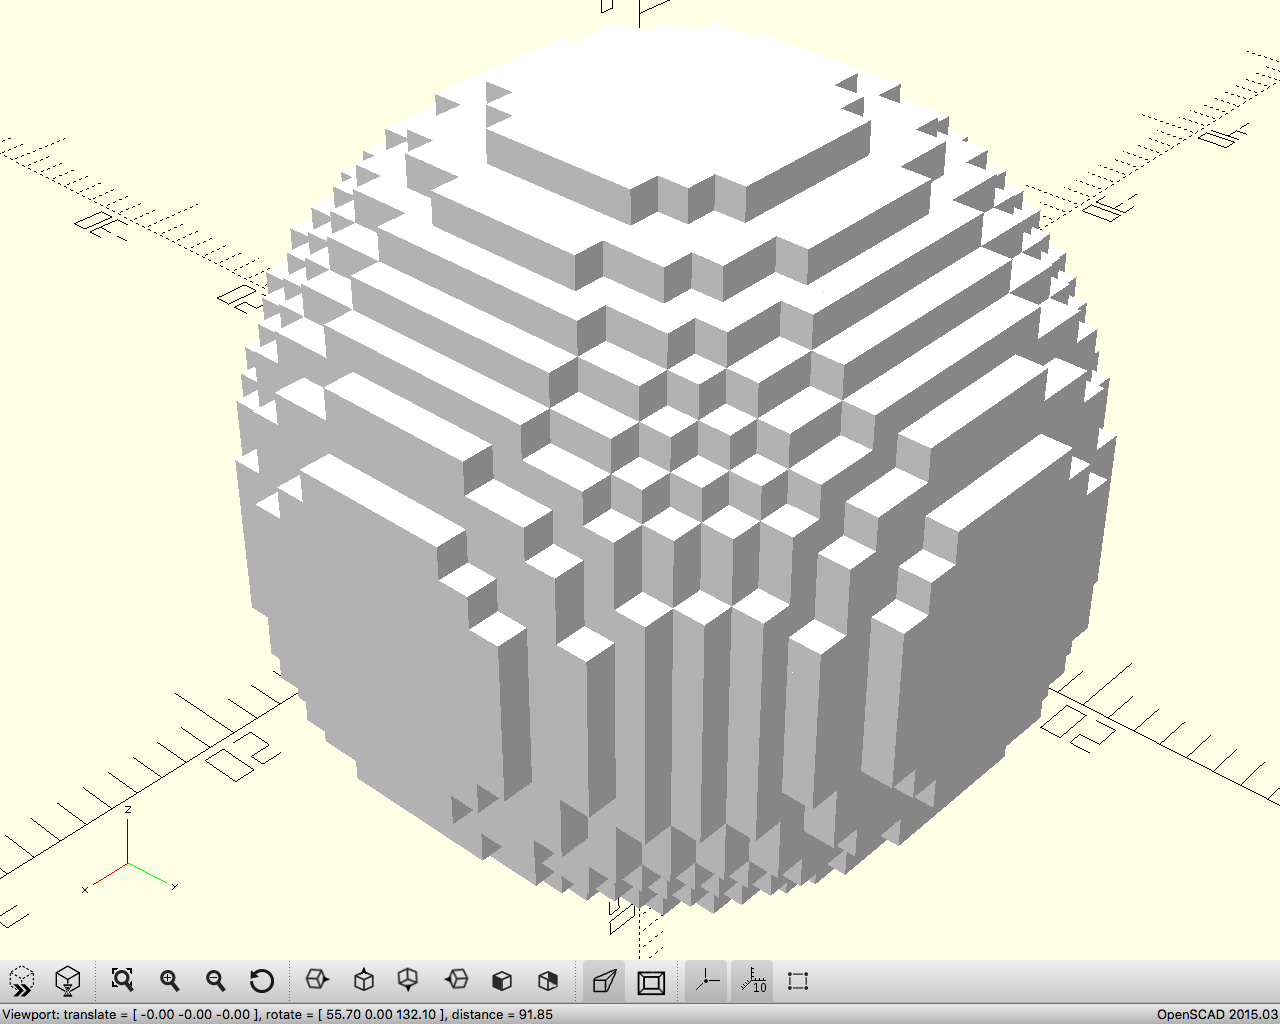
\includegraphics[width=1.0\linewidth]{pic02}
  \caption{Voxelized sphere.}
\label{fig:pic02}
\end{figure}
\FloatBarrier

The genetic algorithm is used with the following parameters:

\begin{table}[h!]
\centering
\label{table01}
\begin{tabular*}{\textwidth}{|c@{\extracolsep{\fill}}|c|}
\hline 
\textbf{Parameter} & \textbf{Value} \\
\hline
\hline
elitism rate & 0.10 \\
\hline
crossover rate & 0.90 \\
\hline
mutation rate & 0.01 \\
\hline
number of individuals & 37 \\
\hline
number of variables &  864 \\
\hline
optimization minutes & 30 \\
\hline
\end{tabular*}
\vspace{2 mm}
\caption{Genetic algorithm parameters.}
\end{table}
\FloatBarrier

\begin{figure}[h!]
  \centering
  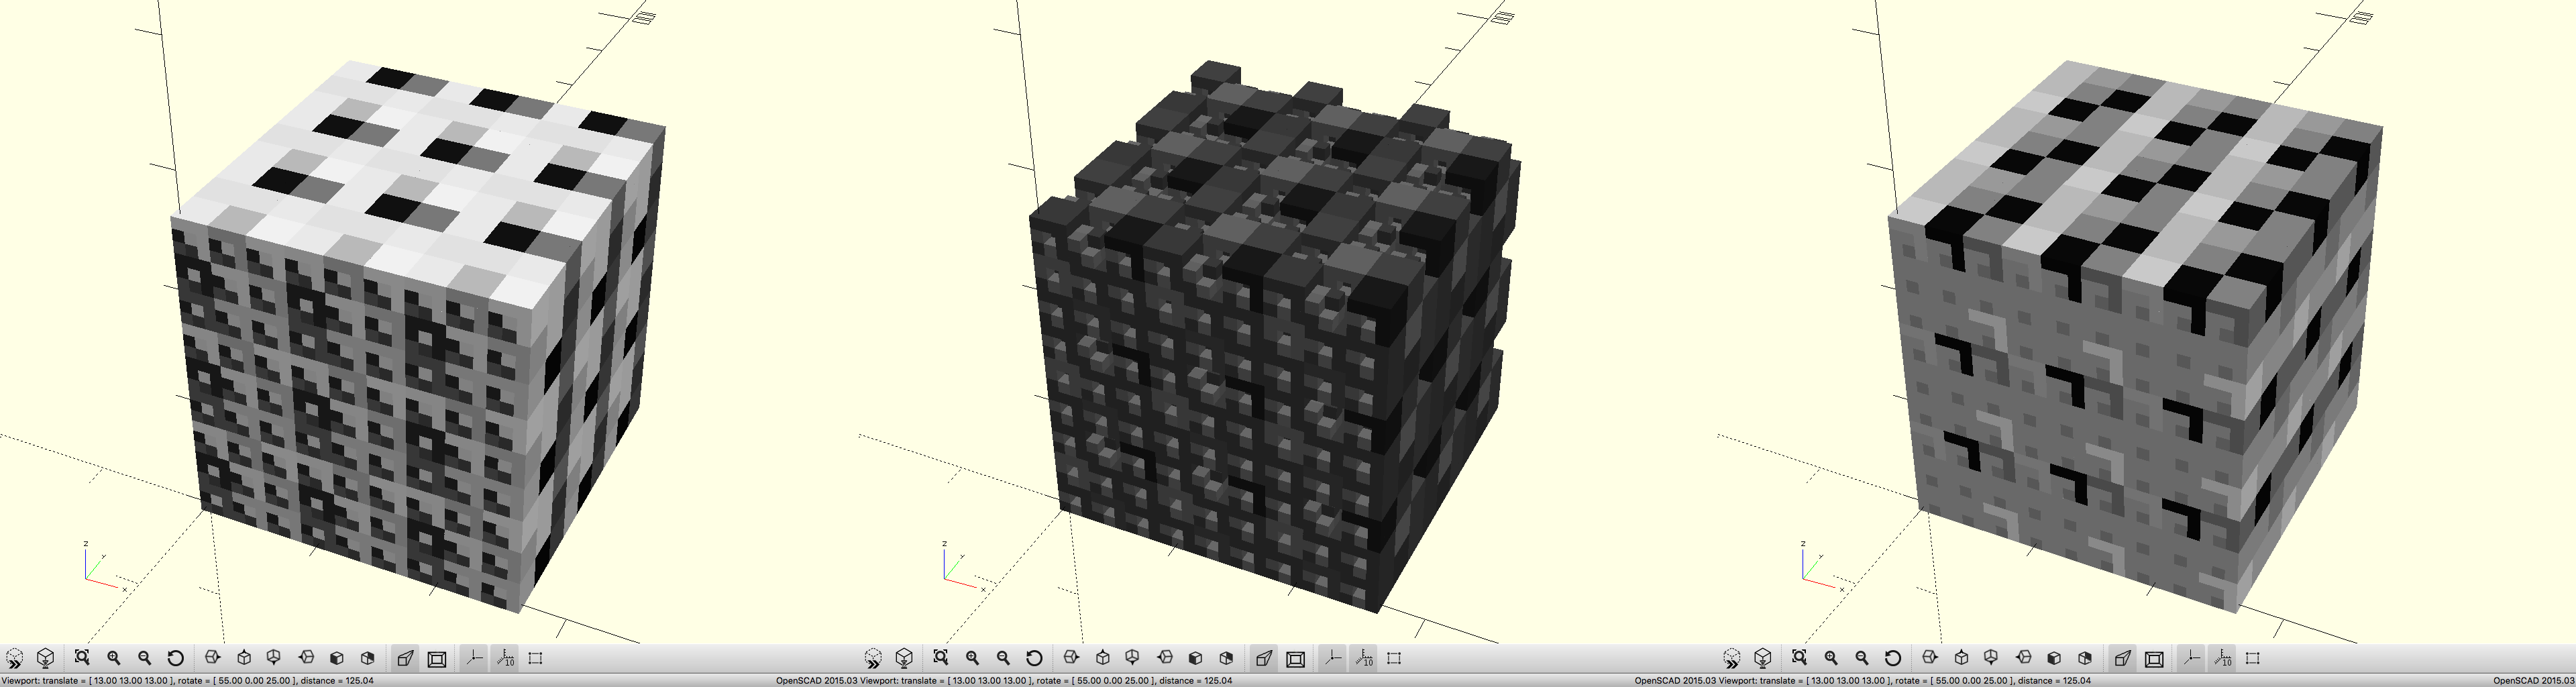
\includegraphics[width=1.0\linewidth]{pic03}
  \caption{Steps taken in the optimization process.}
\label{fig:pic03}
\end{figure}
\FloatBarrier

As it is shown in Fig. \ref{fig:pic03} the optimization process converges much more slower in the 3D space than what was achieved by Hodkinson in the 2D space.

\section{Conclusions} \label{Conclusions}

The extension of the idea for fractal generation from 2D to 3D space shows that in 3D space the process is much more time consuming than in the 2D space. Some speed-ups are possible by parallel implementation of the genetic algorithm \cite{shonkwiler02}. Voxel based representation of 3D objects consumes a lot of computational resources and generated objects are with limited usefulness. A possible application is compression of 3D images, which is similar to the idea of 2D images compression \cite{vences01,albundi01}. Achieved results are promising for further research of the fractal nature of the world in which all we are living. 

%----------------------------------------------------------------------------------------
%   Acknowledgements
%----------------------------------------------------------------------------------------
\section*{Acknowledgements}
This work was supported by private funding of Velbazhd Software LLC.

%----------------------------------------------------------------------------------------
%   Bibliography
%----------------------------------------------------------------------------------------
\begin{thebibliography}{99}

\bibitem{guerin01} Guerin E., Tosan E., \textit{Fractal Inverse Problem: Approximation Formulation and Differential Methods}, In: Levy-Vehel J., Lutton E. (eds) Fractals in Engineering. Springer, London, ISBN 978-1-84628-047-4, 271--285, 2005.

\bibitem{nettleton01} Nettleton D.J., Garigliano R., \textit{Evolutionary algorithms and a fractal inverse problem}, Biosystems, vol. 33, no. 3, ISSN 0303-2647, 221--231, 1994.

\bibitem{ochoa01} Ochoa, G., \textit{On Genetic Algorithms and Lindenmayer Systems}, Parallel Problem Solving from Nature, Lecture Notes in Computer Science, vol. 1498, ISBN 978-3-540-65078-2, 335--344, 1998.

\bibitem{shonkwiler01} Shonkwiler R., Mendivil F., Deliu A., \textit{Genetic Algorithms for the 1-D Fractal Inverse Problem}, Proceedings of the Fourth International Conference on Genetic Algorithms, Morgan Kaufmann, 495--501, 1991.

\bibitem{zelinka01} Zelinka I., \textit{Inverse Fractal Problem. In: Differential Evolution}, Natural Computing Series. Springer, Berlin, Heidelberg, ISBN 978-3-540-20950-8, 479--498 2005.

\bibitem{apache01} The Apache Software Foundation, \textit{Genetic Algorithms - Apache Commons}, http://commons.apache.org/proper/commons-math/userguide/genetics.html , 2018.

\bibitem{printing01} PrintingIn3D, \textit{Printing in 3D - JavaSCAD}, http://www.printingin3d.eu/javascad , 2018.

\bibitem{balabanov01} Balabanov T., \textit{The idea of Jack Hodkinson for fractal generation implemented in 3D version}, http://github.com/TodorBalabanov/Jack-Hodkinson-3D-Fractal , 2018.

\bibitem{shonkwiler02} Shonkwiler R., \textit{Parallel Genetic Algorithms}, Proceedings of the Fifth International Conference on Genetic Algorithms, Morgan Kaufmann, CA, 199--205, 1993.

\bibitem{vences01} Vences L., Rudomin I., Carretera K., Guadalupe L., \textit{Genetic Algorithms for Fractal Image and Image Sequence Compression},  
Proceedings of Comptacion Visual, 35--44, 1997.

\bibitem{albundi01} Al-Bundi S.S., Al-Saidi N.M., Al-Jawari N.J., \textit{Crowding Optimization Method to Improve Fractal Image Compressions Based Iterated Function Systems}, International Journal of Advanced Computer Science and Applications, vol. 7, no. 7, 392--401, 2016.

\end{thebibliography}

\end{document}
